\newpage
\section{Appendix A}
\label{sec:Appendix A}

\subsection{Payload Dimensions}
\begin{figure}[!h]
\begin{center}
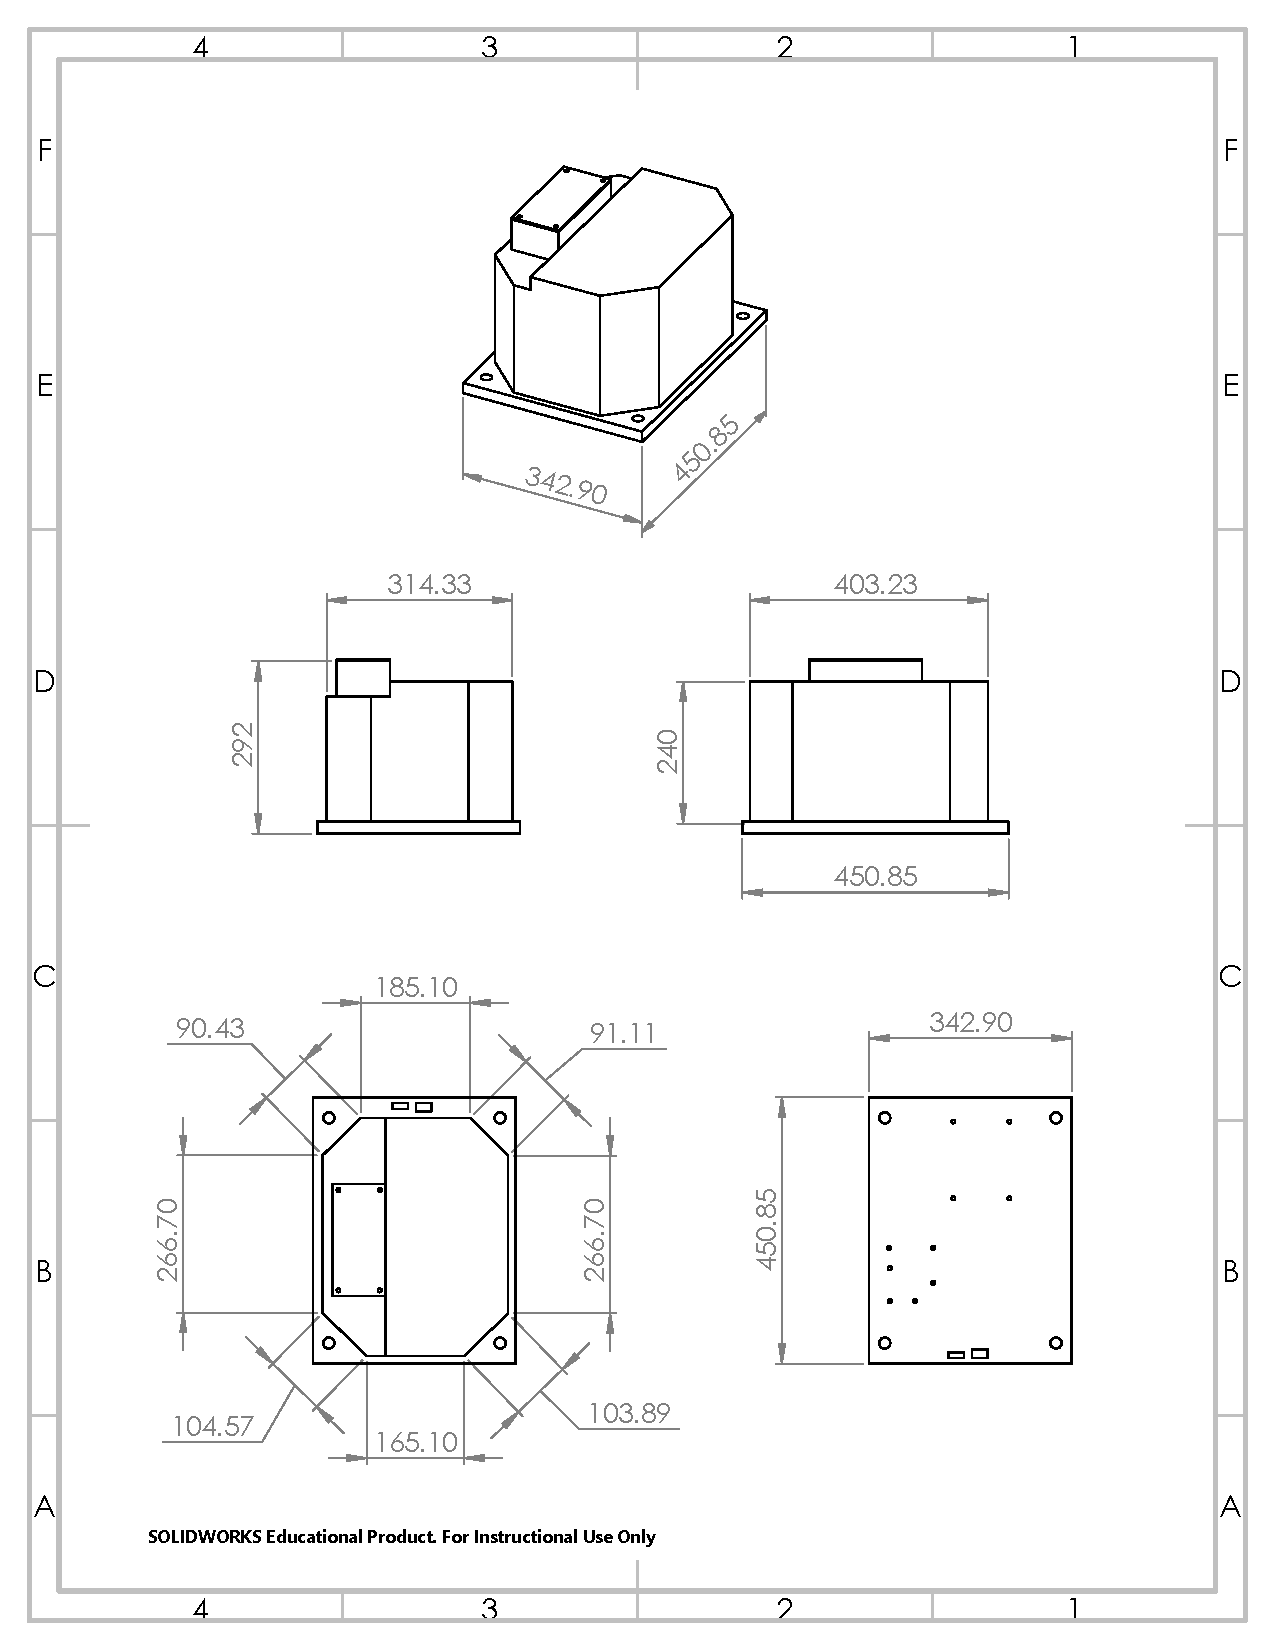
\includegraphics[scale=.6]{./Figures/Payload_Dim.pdf}
\caption{Payload dimensions in millimeters including mounting holes.}
\label{fig:payload_dim}
\end{center}
\end{figure}

\newpage
\subsection{Astrobiology Methods and Testing}

We realize that the flow rate is very low, however we are interested in doubling our intake and perfecting our methodology in conjunction with improved assembly and post-flight sanitization procedures. If we obtain definitive results then our goal is to pursue opportunities that would allow us to reproduce the methodology on a larger scale.

We have decided on an alternative approach to the SMITH sterilization procedures.  For our last flight we assembled the payload and decontaminated it two different clean rooms.  This year, for the both assembly and decontamination we will use the same clean room.  All equipment used in the assembly process will either be autoclaved or taken from previously unopened sanitized packaging. The autoclaved, pre-sanitized items and the clean box will be washed in a 70 \% ethanol solution before being placed inside a SterilGARD e3 Class II Biological Safety Cabinet. The Cabinet has a laminar flow air barrier and UV lights built into the ceiling for decontaminating the workspace prior to use.

For post flight decontamination, all equipment used in the filtration process will either autoclaved or taken from previously unopened sanitized packaging. The autoclaved, pre-sanitized items and the clean box will be washed in a 70 \% ethanol solution before they are placed inside the same SterilGARD e3 Class II Biological Safety Cabinet used during assembly. Both the control and sample collection solutions will be vacuum filtered through a Fluropore membrane filter (13 mm; 0.22 micron) to collect specimens on the filter surface. The filters will be packaged for shipment to RTL Genomics [17] for 16S ribosomal RNA sequencing. All post flight sanitation and sample and control filtration procedures will take place under the supervision of Professor Donna Pattison from the Department of Biology and Biochemistry at The University of Houston.  Also, with regard to the flow rate, we were able to measure a flow rate of AAAAA in our vacuum chamber set up; pressure conditions were AAAAA and temperature was measured at AAAAA. The microbe count was provided in a histogram style chart; going forward exact total counts will be reported as well.


The intent behind the culturing is to provide an additional means for float and ground analysis but mainly to attempt culturing the microbes under varied conditions. We aim to address the question of future sequencing results mirroring background or ground population between Houston and New Mexico by: collecting and analyzing samples from various points on our payload in Houston, New Mexico and from the the filters attached to the inside of our payload during the journey between the two states. We will also run the collection system in the clean room for ten hours to simulate flight time and analyze the results to obtain a background reading.

\newpage
\subsection{Flight Computer and Electronic Diagrams}

%\subsection{Power Distribution}
\begin{figure}[!h]
\begin{center}
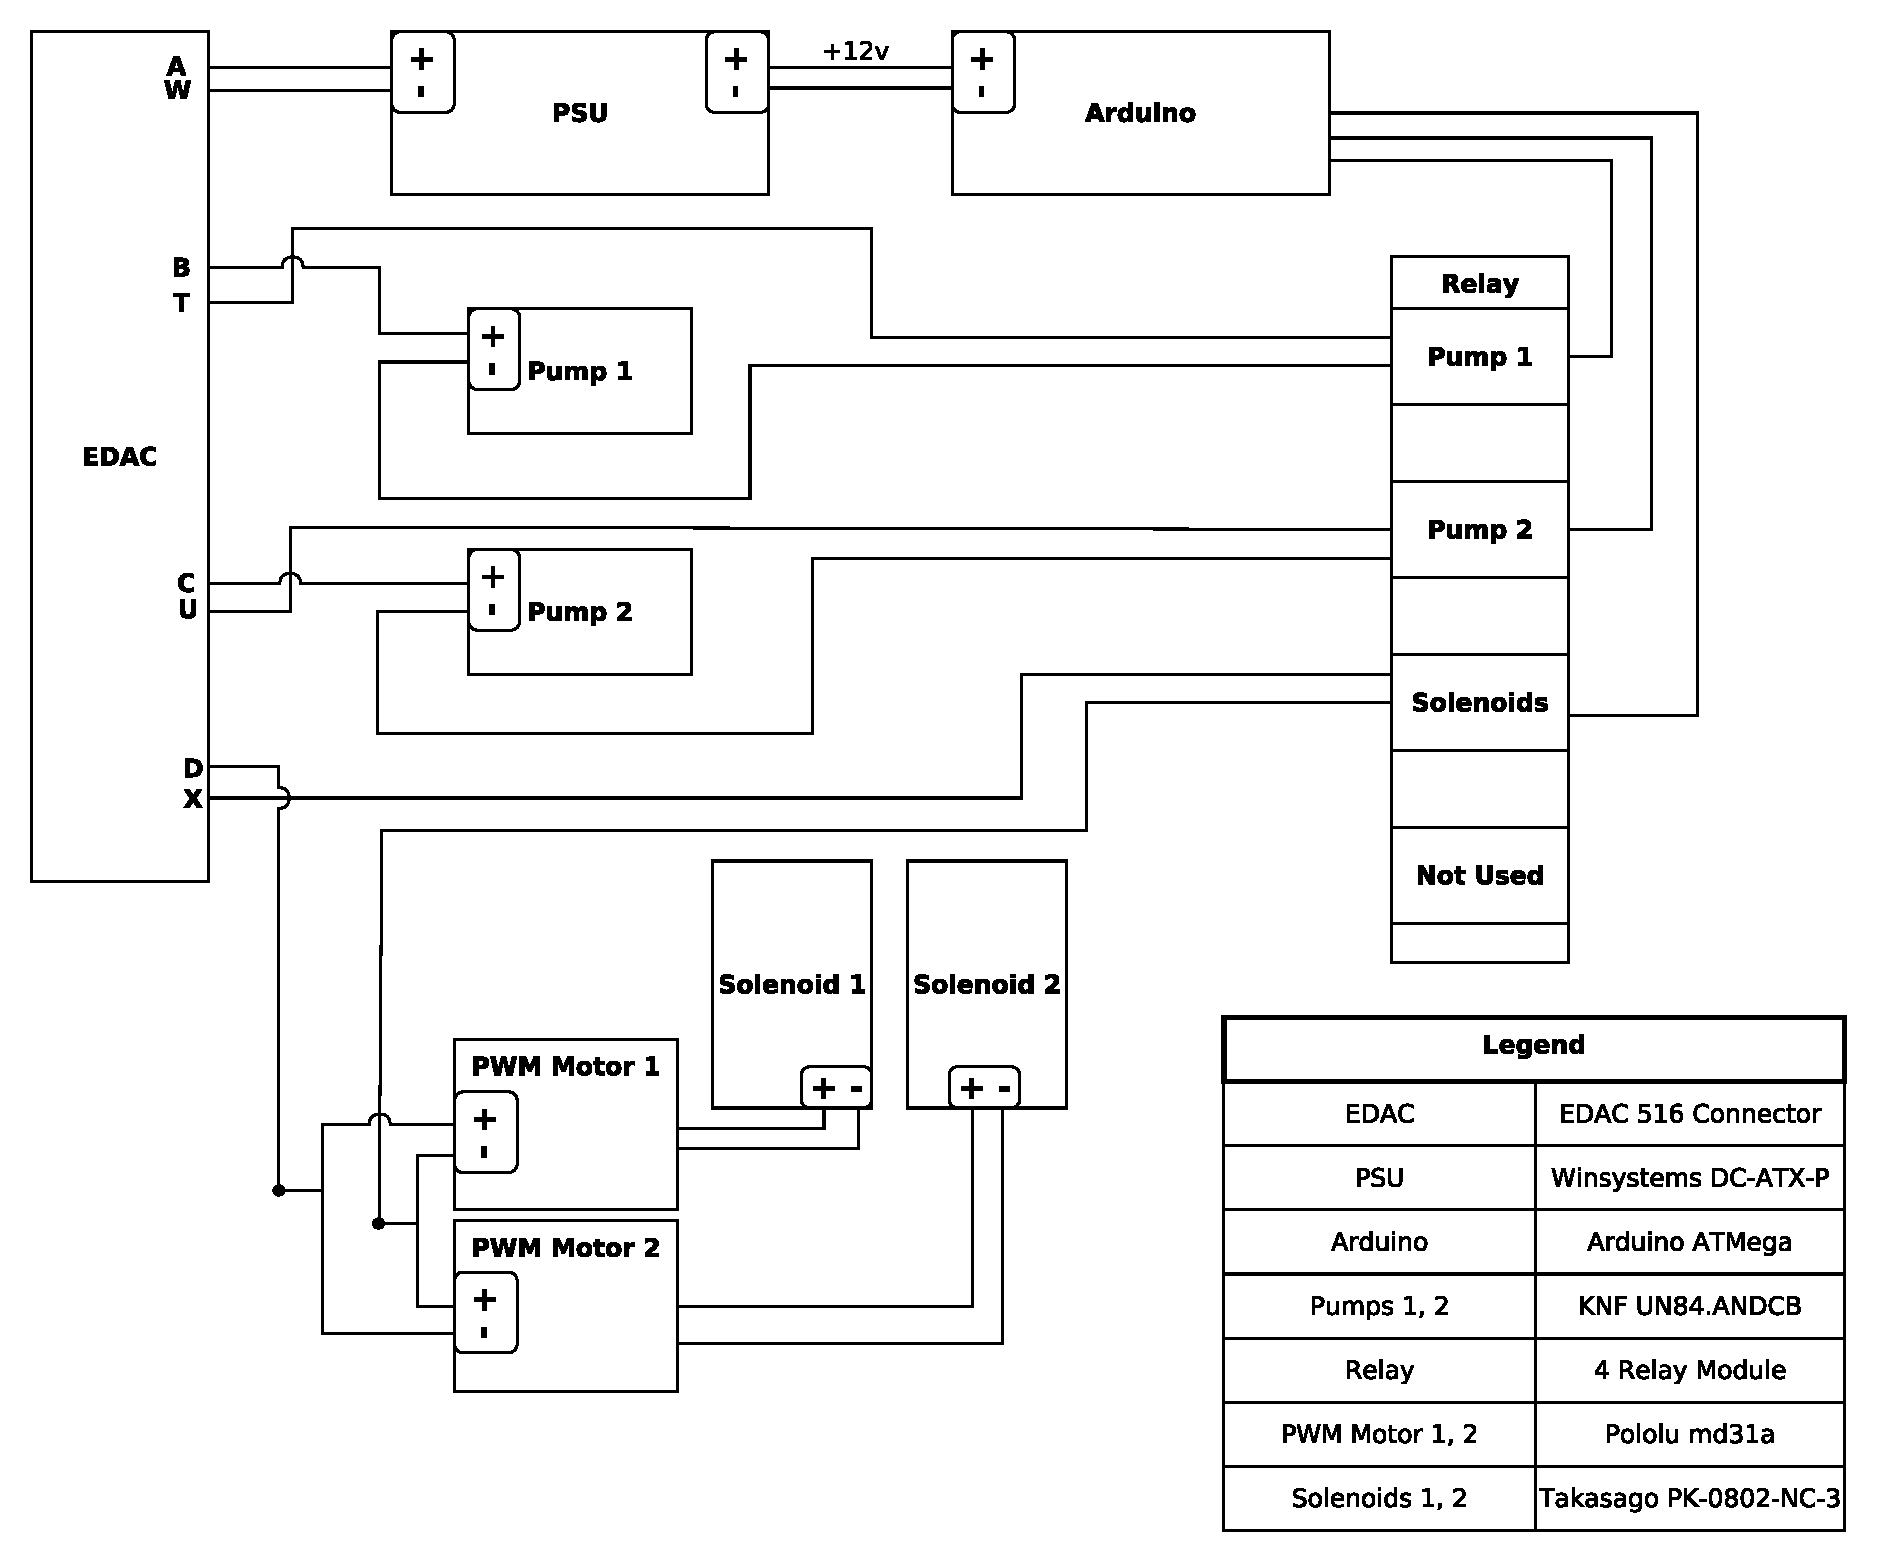
\includegraphics[scale=.5]{./Figures/power-distro.pdf}
\caption{General power distribution diagram.}
\label{fig:power-distro}
\end{center}
\end{figure}

\newpage
%\subsection{Flight Computer Battery Design}
\begin{figure}[!h]
\begin{center}
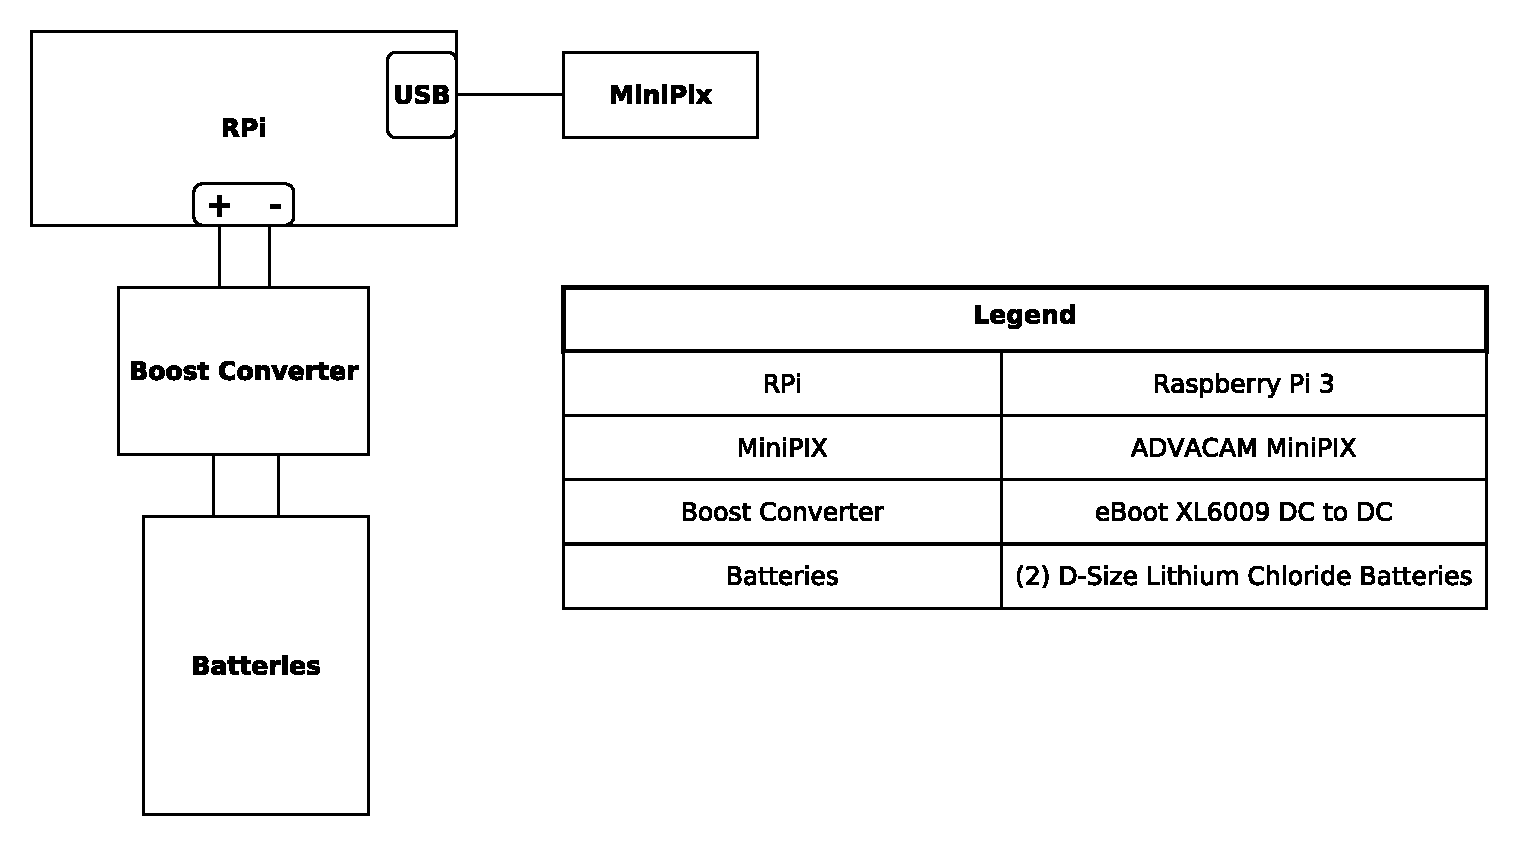
\includegraphics[scale=.5]{./Figures/rpi-batteries.pdf}
\caption{Concept schematics with batteries we will attempt to use in flight.}
\label{fig:rpi-batteries}
\end{center}
\end{figure}

\newpage
\subsection{Integration and Flight Information}

Currently, the seven members will travel to integration and flight.  Currently,
the integration and flight team will consist of Fre'Etta Brooks, Steven Oliver, Andrew Walker,
Kevin Portillo, Reed Masek, Andrew Renshaw and Samuel Garcia Morelos.

%\newpage
%\subsection{Additional Payload Information}
\textbf{Payload Orientation:} We request to have the same payload orientation as the 2017 mission.
We will require one of our walls to be facing the outside and have no obstructions.

%\subsection{Payload Top View}
\begin{figure}[!h]
\begin{center}
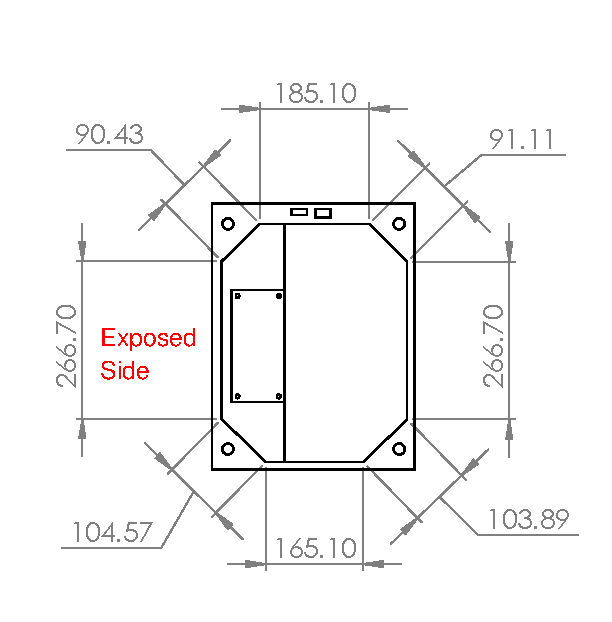
\includegraphics[scale=.4]{./Figures/PayloadTop_red.pdf}
\caption{The red text highlights the side that must be exposed to the outside.}
\label{fig:PayloadTop}
\end{center}
\end{figure}

\textbf{Discrete Channels:} if possible, we will require the use of discrete channels.
We are discussing the possible use of discrete channels and would like to test our designs at integration.
We will update and provide further documentation as our design is finalized.
